Um in die Einstellungen für die Monitore zu gelangen, klicken Sie im \enquote{Data-Input-Menü} auf den Punkt \enquote{Monitore verwalten} (siehe Abbildung \ref{menu-data-input}).\\
\\
\begin{figure}[H]
\centering
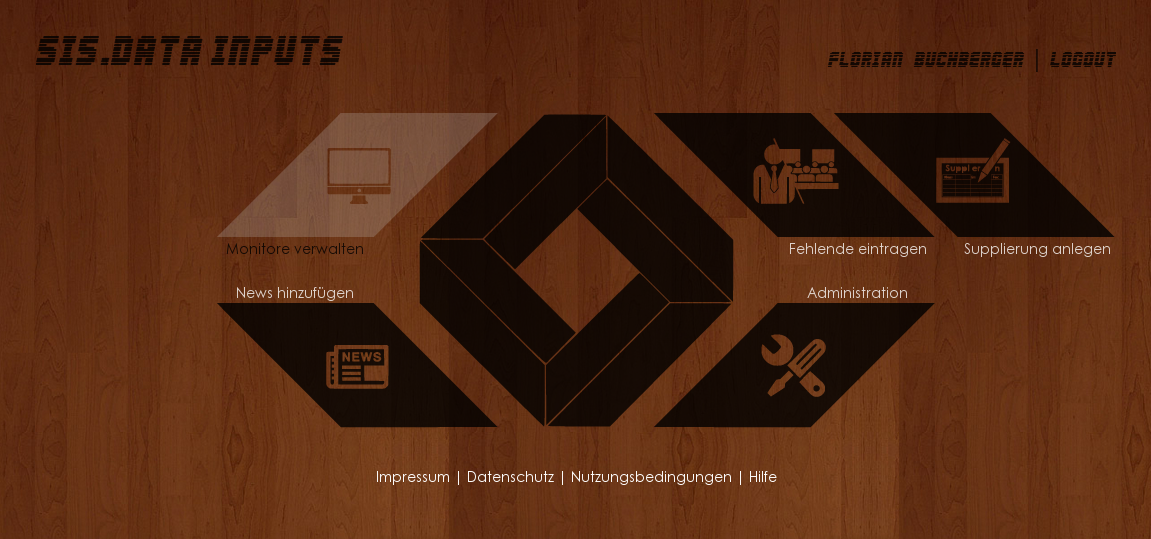
\includegraphics[keepaspectratio=true, width=14cm]{images/screenshots/data-inputs.png}
\label{menu-data-input}
\caption{Data-Input-Menü}
\end{figure}
Nach dem Öffnen der Seite werden oben im Fenster die aktiven Monitore aufgelistet. Darunter sind die Einstellungen zu finden.\\
\\
\begin{figure}[H]
\centering
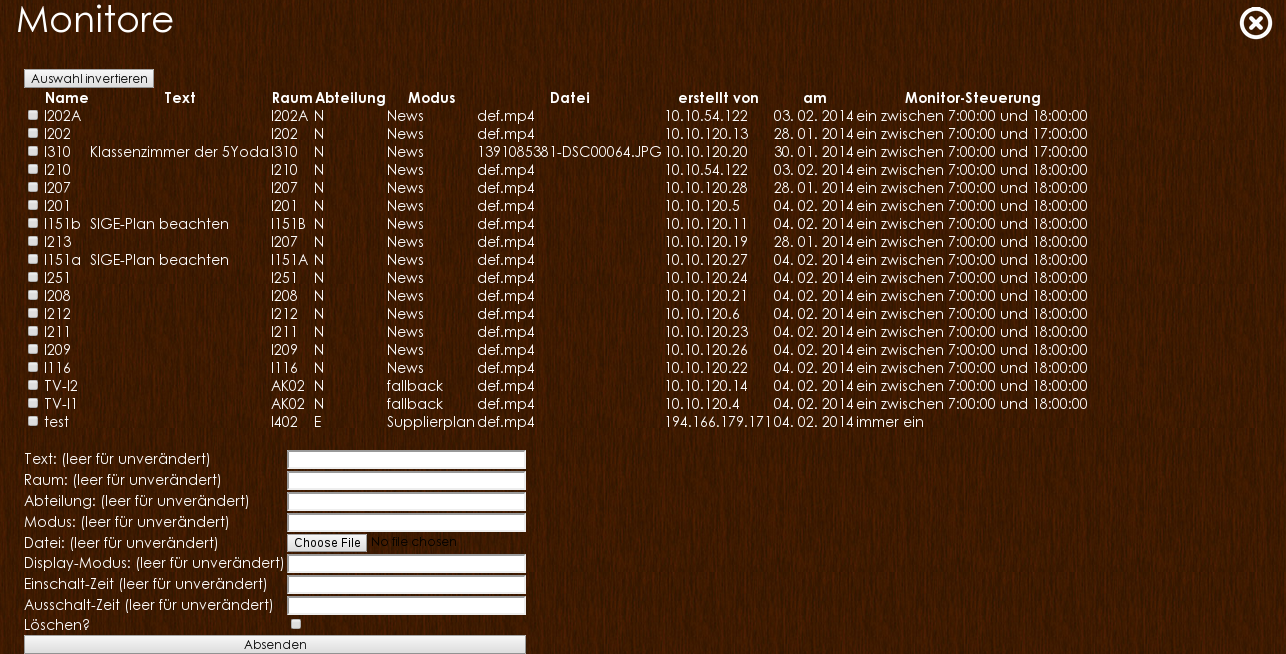
\includegraphics[keepaspectratio=true, width=14cm]{images/screenshots/monitors.png}
\label{monitors}
\caption{Monitor-Einstellungen}
\end{figure}
Die Monitore, deren Einstellungen verändert werden sollen, müssen mit einem Klick auf die Checkbox links neben der Anzeige ausgwählt werden. Es können mehrere ausgewählt werden. Mit dem Button \enquote{Auswahl invertieren} werden alle gesetzten Checkbox rückgesetzt, und umgekehrt.
\\
\subsection{Hinzufügen}

Ein neuer Monitor kann nicht über das Web-Interface hinzugefügt werden, die Monitore registrieren sich selbstständig am Server. Nach der Registrierung stehen sie zur Verwaltung zur Verfügung.

\subsection{Entfernen}

Um einen Monitor aus der Liste der aktiven Monitore zu entfernen, wähle den jeweiligen Monitor über die Checkbox aus, setze die \enquote{Löschen?}-Checkbox und klicke auf \enquote{Änderungen anwenden}.

\subsection{Text verändern}

Der Text, der am linken unterem Eck des Monitors kann über das Eingabefeld \enquote{Text} geändert werden. Wird das Feld leer gelassen, so wird der alte Wert beibehalten.\\
\textit{Achtung:} Leerzeichen werden nicht als leer erkannt.

\subsection{Raum verändern}

Für die Darstellung des Stundenplanes des jeweiligen Raumes wird jedem Monitor ein Raum zugeordnet. Diese Einstellung kann über das Eingabefeld \enquote{Raum} angepasst werden. Durch Doppelklick auf das Eingabefeld öffnet sich - sofern der verwendete Browser diese Funktion unterstützt - ein Menü, in dem durch Eingeben gesucht werden kann. Wird das Feld leer gelassen, so wird der alte Wert beibehalten.

\subsection{Abteilung verändern}

Die News können Abteilungen zugeordnet werden. Ebenso ist der Supplierplan für jede Abteilung anders. Als Folge daraus gibt es eine Einstellungsmöglichkeit für die Abteilung. Durch Doppelklick auf das Eingabefeld öffnet sich - sofern der verwendete Browser diese Funktion unterstützt - ein Menü, in dem durch Eingeben gesucht werden kann. Wird das Feld leer gelasen, so wird der alte Wert beibehalten.

\subsection{Modus verändern}

Um die ausgewählten Monitore auf Supplierplan, Stundenplan, News etc. umzuschalten, wird das Eingabefeld \enquote{Modus} verwendet. In diesem Feld sind folgende Werte zulässig:
\begin{itemize}
	\item News
	\item Stundenplan
	\item Supplierplan
	\item Supplierplan \& News
	\item Bild
	\item (Video)
	\item (fallback)
\end{itemize}
Durch Doppelklick auf das Eingabefeld öffnet sich - sofern der verwendete Browser diese Funktion unterstützt - ein Menü mit den möglichen Werten. Wird das Feld leer gelassen, so wird der alte Wert beibehalten.\\
\\
Der Modus \enquote{Video} ist zwar implementiert, allerdings ist der Raspberry Pi nicht in der Lage, die Videos wiederzugeben.\\
Der Modus \enquote{fallback} fährt den Monitor auf das FTKL-Schnitzel-Suppla-Projekt. 
\textit{Beachte:} Es ist nicht über das Interface möglich, den Monitor wieder auf das SIS-Projekt zurückzuholen.

\subsection{Datei verändern}

Für die Modi \enquote{Bild} und \enquote{Video} muss eine Datei hochgeladen werden, welche dann angezeigt wird.\\ 
Unterstützte Dateitypen sind:
\begin{itemize}
	\item JPG, JPEG
	\item PNG
	\item GIF
	\item MP4, MPEG
\end{itemize}
Die maximale Dateigröße ist limitiert durch:
\begin{itemize}
	\item das Upload-Script auf 800 MB
	\item das Upload-HTML-Tag auf 800 MB
	\item die PHP-Konfiguration am Server (Stand: 2014-02-28) auf 128 MB
\end{itemize}
 